%Template v.1.0: Taylor Arnold and Simon Gabay, december 2025
% CECI EST UN FICHIER DE MODÈLE LATEX POUR LES ARTICLES INCLUS DANS
% *Anthology of Computers and the Humanities*. AJOUTEZ L'OPTION
% 'final' LORS DE LA CRÉATION DE LA VERSION FINALE DE L'ARTICLE. 
% NE PAS modifier la classe du document
\documentclass[final, fra]{anthology-ch}     % pour la version finale
%\documentclass[fra, custom]{anthology-ch}      % pour la soumission

% CHARGER LES PACKAGES LaTeX
\usepackage{booktabs}
\usepackage{graphicx}
\usepackage{subcaption} % pour les sous-figures
\usepackage{wrapfig} % pour les figures dans le §
\usepackage{fontspec}
\usepackage{tabularx}
\usepackage{threeparttable}
\usepackage{makecell}


% AJOUTEZ vos propres packages avec \usepackage{}

% TITRE DE LA SOUMISSION
% Remplacez ceci par le titre de votre soumission
\title{Déserter des troupes coloniales~? Cadre juridique et comportements (Caraïbe française, \textsc{xviii}\textsuperscript{e} siècle)}

% INFORMATIONS SUR LES AUTEURS ET LES AFFILIATIONS
% Pour chaque auteur, utilisez une nouvelle commande \author, avec
% les numéros entre crochets indiquant les affiliations correspondantes
% (section suivante) et l'ORCID-ID pour chaque auteur.  
\author[1]{Elodie Bascoul}[
  orcid=0009-0002-7324-6469,
  email=elodie.bascoul@unige.ch
]

\author[1]{Marion Philip}[
  orcid=0009-0001-6846-2688,
  email=marion.philip@unige.ch
]

\author[1]{Méloé Maillard}[
  orcid=,
  email=méloé.maillard@unige.ch
]

\author[1]{Simon Gabay}[
  orcid=0000-0001-9094-4475,
  email=simon.gabay@unige.ch
]

\author[1]{Marie Houllemare}[
  orcid=0000-0002-9120-8944,
  email=marie.houllemare@unige.ch
]

% Bien que nous encouragions l'ajout des ORCID-ID pour tous les auteurs, 
% vous pouvez inclure des auteurs qui n'en ont pas en laissant le champ vide.
%\author[1]{Auteur Trois}[
%  orcid=
%]

% Il doit y avoir un appel à \affiliation pour chaque affiliation des auteurs.
% Plusieurs affiliations peuvent être attribuées à un auteur
% et une affiliation peut être attribuée à plusieurs auteurs. 
\affiliation{1}{Université de Genève, Suisse}

% MOTS-CLÉS
% Fournissez un ou plusieurs mots-clés séparés par des virgules
% en utilisant les commandes suivantes
\keywords[fra]{Reconnaissance automatique de texte (ATR), désertion, Caraïbe française (\textsc{xviii}\textsuperscript{e} siècle), législation militaire}
\keywords[eng]{Automatic Text Recognition (ATR), desertion, French Caribbean (\textsc{18}\textsuperscript{th} century), military legislation}

% MÉTADONNÉES DE LA PUBLICATION
% Ces champs seront remplis lors de la publication ; 
% ils peuvent être laissés par défaut lors de la soumission
\pubyear{2026}
\pubvolume{4}
\pagestart{27}
\pageend{36}
\paperorder{4}
\conferencename{Actes de la Conférence Humanistica}
\conferenceeditors{Serena Crespi, Simon Gabay, Martin Grandjean, Ariane Pinche, Marie Puren et Léa Saint-Raymond}
\doi{10.63744/ZkpxSmLJdwIB}
\customhead{}

\addbibresource{bibliography.bib}

%%%%%%%%%%%%%%%%%%%%%%%%%%%%%%%%%%%%%%%%%%%%%%%%%%%%%%%%%%%%%%%%%%%%%%%%%%%
% DÉBUT DU TEXTE
\begin{document}
\maketitle

\begin{abstract}
Military desertion in the French Caribbean during the eighteenth century constitutes a privileged vantage point for examining the effects of normative change on individual behavior. By mobilizing automatic text recognition and layout analysis models specifically trained on handwritten colonial archives, this research analyzes an original corpus of 127 judicial case files concerning deserter soldiers. The quantitative and qualitative exploitation of these sources reveals a significant correlation between the royal ordinance of 1776 (which replaced capital punishment with forced labor) and a measurable increase in acts of desertion, particularly pronounced in Saint-Domingue. These findings suggest that the relative mitigation of punishment altered soldiers’ risk calculations, thereby revealing the sensitivity of individual practices to transformations in the legal framework. The study contributes both to the history of colonial penal systems and to the use of computational methods in social history.
\end{abstract}

\section{Introduction}

\begin{wrapfigure}{r}{0.5\textwidth}
    \centering
    \vspace{-.5cm}
    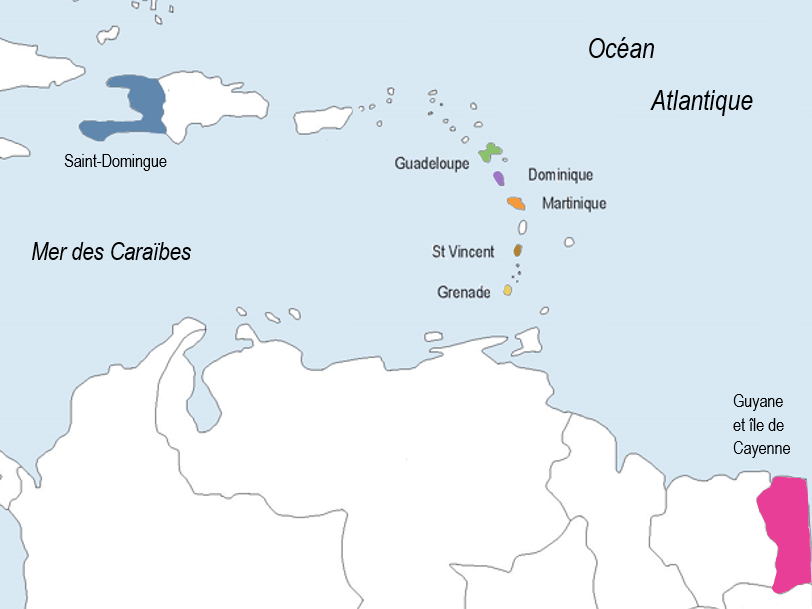
\includegraphics[width=.95\linewidth]{images/Les Antilles françaises au XVIIIe s.PNG}
    \caption{La Caraïbe française au \textsc{xviii}\textsuperscript{e} siècle. (Couleurs attribuées selon la Fig.~\ref{fig:desertions-annee}).}
    \label{fig:carte-antilles-fr-xviiie}
    \vspace{-.5cm}
\end{wrapfigure}

Phénomène massif à l'époque moderne, la désertion est considérée comme une véritable \og maladie des armées \fg{} \cite{CorvisierAndré1971Smem}. Est réputé déserteur en France et dans les colonies de la Caraïbe française du \textsc{xviii}\textsuperscript{e} siècle quiconque s'éloigne de plus de deux lieues de sa garnison sans un congé \footnote{\textit{Ordonnance du Roy, portant amnistie générale […] \& qui impose la peine de mort aux déserteurs, du 2 juillet 1716}, Chez François Reynier, imprimeur du Roy à Perpignan, 1719.  Articles III et IV, pp. 5-6.}. Les déserteurs rattrapés sont punis par les conseils de guerre,
qui appliquent les peines prévues par les ordonnances royales.
%EB: Ceux qui ne sont pas rattrapés sont jugés par contumace, ce qui signifie que s'ils sont un jour rattrapés, la peine sera exécutée sans nouveau jugement.
%SG: Retirer "ainsi"->pas de lien de conséquence avec la phrase précédente
Si les documents judiciaires traitant de la désertion prennent plusieurs formes juridiques (procès criminel, jugement contradictoire, jugement par contumace, compte-rendu du conseil de guerre, etc.), ils possèdent cependant tous des informations communes, que le soldat en fuite ait été appréhendé ou non~: son nom, son régiment et la date de sa fuite. C'est cette dernière information que nous souhaitons exploiter.
%SG: conclut ton raisonnement: "ce sont ces informations que nous voulons exploiter" ou truc du genre

%L'historiographie de la Caraïbe française à l'époque moderne (fig.~\ref{fig:carte-antilles-fr-xviiie}) a déjà fourni plusieurs analyses: des études quantitatives se sont concentrées sur les esclaves, portant notamment sur la traite transatlantique\footnote{Voir le projet \textit{Slave Voyages}, \url{https://www.slavevoyages.org}.} et sur le marronnage \cite{EddinsRunaways}, mais aucune étude d'envergure sur les troupes coloniales n'a encore été menée\footnote{Des études ont été menées, mais non de manière quantitative, comme ceux de Boris Lesueur \cite{lesueur_troupes_2009,lesueur_troupes_2015}.}. 
%SG: la phrase est mal tournée. Je propose: 
Si l'étude de la Caraïbe française à l'époque moderne (Fig.~\ref{fig:carte-antilles-fr-xviiie}) a déjà connu un tournant quantitatif, celui-ci a surtout concerné les recherches sur les esclaves, et tout particulièrement la traite transatlantique (\href{https://www.slavevoyages.org/}{Slave Voyages}) et le marronnage \cite{EddinsRunaways}. Les troupes coloniales, en revanche, attendent toujours des travaux de ce type \footnote{Des études ont été menées, mais non de manière quantitative. Voir \cite{lesueur_troupes_2009,lesueur_troupes_2015}}. 
%Pourtant, 
%SG: fais attention à tes connecteurs logiques. "pourtant" est impropre ici, car il n'y a pas de concessive ensuite mais une poursuite du raisonnement: tu abandonnes la question quantitative des soldats pour passer à la question des évolutions juridiques. 
Étudier les dynamiques de fuite des soldats au regard des évolutions juridiques dans les années 1770 peut être utile : elle permet de se demander s'il y a une corrélation entre le changement du droit et le changement dans la pratique des individus, sur une échelle de plusieurs dizaines d'années.
%Elle permet en effet d'observer un phénomène de corrélation entre le changement du droit et de changement dans la pratique des individus, sur une échelle de plusieurs dizaines d'années.
%SG: tu ne peux pas donner la réponse avant de poser la question! Ca permet de se demander s'il y a une corrélation et comment l'observer
Dans quelle mesure une mutation juridique peut-elle changer le comportement de personnes?
%SG: eviter les questions par comment. Dans quelle mesure? Je ne suis pas sûr que le droit "mute": on comprend mais c'est un peur border. Le droit "change" et les gens "s'adaptent au changement"
Quel impact peut-elle avoir sur les pratiques de la désertion? 
%SG: en quoi "stratégie de désertion" est-il différent de "pratique"? tu coordonnes deux objets de niveaux différents, le second reprenant pour partie le premier. D'ailleurs, ton papier ne va pas traiter des stratégies de désertion, mais juste de la fréquence des désertions, en montrant in fine que ce n'en sont pas toujours "des vraies"


%SG: ça vient trop tôt. D'abord tu dis ce que tu veux faire, et ensuite tu proposes une méthode.
%Avec cette étude multiscalaire nous souhaitons montrer que l'abolition de la peine de mort pour les déserteurs dans la Caraïbe française au \textsc{xviii}\textsuperscript{e} siècle précipite de nombreuses désertions, et que la connaissance de la norme et de ses modifications influence le comportement des soldats à une échelle individuelle.
%SG: je propose: 
En étudiant les dossiers individuels de déserteurs dans la Caraïbe française, nous pensons être en mesure de prouver qu'une accélération des désertions à la fin du \textsc{xviii}\textsuperscript{e} siècle est fortement corrélée à un changement dans la législation. Cette première affirmation faite sur une base purement quantitative doit cependant être nuancée par l'analyse qualitative de quelques cas individuels, rappelant l'importance d'une analyse multiscalaire. Ce travail permet ainsi de contribuer à l'étude des réactions individuelles face aux changements dans le droit.
%SG: Un truc du genre "Ce travail permet ainsi de contribuer à l'étude des réactions individuelles face aux changements dans le droit" me paraît plus propre à la conclusion, où tu "élèves" le débat. Garde des billes pour la fin, surtout si tu as peu de mots.


\section{État de l'art}

Récemment, plusieurs projets en histoire moderne coloniale ont été consacrés à des populations subalternes qui laissent peu de trace dans les archives, tels les esclaves. 
%Dans ses travaux sur l’affranchissement, L. Chappuis a ajusté le modèle de reconnaissance automatique de textes (\textit{Automatic Text Recognition}, ATR) \texttt{FoNDUE-GD} \cite{vers-un-modele-diachronique-pour-les-mains-modernes-françaises} afin de l’adapter à ses données, pour utiliser la lecture distante sur des testaments de planteurs propriétaires d’esclaves à l’Île de France (actuelle Île Maurice). 
%SG: l'articulation est imparfaite: on utilise pas la LD en ajustant un modèle. On ajuste un modèle pour extraire des données, et ces données sont utilisées pour visualisation le résultat 
%Elle a pu découvrir que les esclaves affranchis sont majoritairement des femmes, et en particulier celles qui travaillent au plus près du maître en tant que domestique, partageant une intimité quotidienne avec eux \cite{loraine-chappuis-ile-de-france}.
%SG: je propose: 
Dans ses travaux sur l’affranchissement, L. Chappuis a ajusté le modèle de reconnaissance automatique de textes (\textit{Automatic Text Recognition}, ATR) \texttt{FoNDUE-GD} \cite{vers-un-modele-diachronique-pour-les-mains-modernes-françaises} aux testaments de planteurs propriétaires d’esclaves à l’Île de France (actuelle Île Maurice). En visualisant les données ainsi extraites par le biais d'une carte, elle a pu démontrer que les esclaves affranchis sont majoritairement des femmes qui travaillent au plus près du maître, partageant une intimité quotidienne avec eux \cite{loraine-chappuis-ile-de-france}.
Cr. Eddins, quant à elle, a étudié les annonces de dénonciation et de recherche des esclaves en fuite dans le journal imprimé de Saint Domingue \textit{Les Affiches américaines}. Elle a ainsi démontré que l’insertion sociale des esclaves nés à Saint-Domingue et les liens entre plantations leur permettaient de fuir plus longtemps et de manière plus efficace que les esclaves arrivés d’Afrique. L'organisation de la fuite et la survie au sein des communautés marronnes de Saint-Domingue seraient ainsi les prémices d'une conscience collective menant à la Révolution haïtienne \cite{EddinsRunaways}. 

Les projets portant sur les archives coloniales utilisent des jeux de données de plus en plus conséquents, faisant de la création et de l’amélioration des modèles d'ATR de véritables enjeux pour simplifier l’accès aux ressources historiques. C'est notamment le cas du projet Globalise Time Machine Europe, qui développe une démarche d’histoire globale en utilisant les archives de la Compagnie des Indes Néerlandaises \cite{a-digital-infrastructure-for-the-voc-archives}.

Dans nos archives manuscrites du \textsc{xviii}\textsuperscript{e} siècle, il est désormais difficile de se passer de l’utilisation de l'ATR, qui permet d’accélérer le repérage de thématiques et d’informations ciblées dans les archives. Ainsi, en matière d’ATR, plusieurs choix s’offrent à nous. La plateforme Transkribus \cite{transkribus-a-service-plateform} propose un modèle pour les mains du \textsc{xviii}\textsuperscript{e} siècle, mais son utilisation est payante. Gratuit et ouvert, Kraken \cite{escriptorium-an-open-source-platform} propose depuis plusieurs années des modèles pour les mains françaises de plus en plus précis. L’amélioration de ces modèles est rendue possible grâce à l’utilisation de divers jeux de données distribués selon les recommandations de HTR United \cite{htr-united-a-solution-towards-a-common}. Leur agrégation pour les entraînements fait émerger des modèles toujours plus conséquents, généraux et performants \cite{vers-un-modele-diachronique-pour-les-mains-modernes-françaises,transcribing-western-modern-manuscripts}.

\section{Entraînement}

Nous avons été confrontés à deux problèmes. D'une part, la nature très diversifiée des documents (correspondance, formulaires, comptes-rendus, etc., fig.~\ref{fig:trois_images}) multiplie les problèmes de mise en page (passages imprimés, notes marginales, etc.). D'autre part, nos sources sont écrites par de très nombreuses personnes, qui ont toutes leur propre main. Afin d'extraire l'information des fac-similés numériques, il a donc été nécessaire de créer deux modèles: un premier d'analyse de mise en page, et un second d'ATR \footnote{Ces deux modèles ont été pensés et créés conjointement dans le cadre du projet de recherche ~\href{https://github.com/Masculinites-Esclavagistes/MEGV-FR-MSS-18}{MEGV}
.}.

\vspace{.2cm}
\begin{figure}[ht]
\centering

\begin{subfigure}{0.32\textwidth}
    \centering
    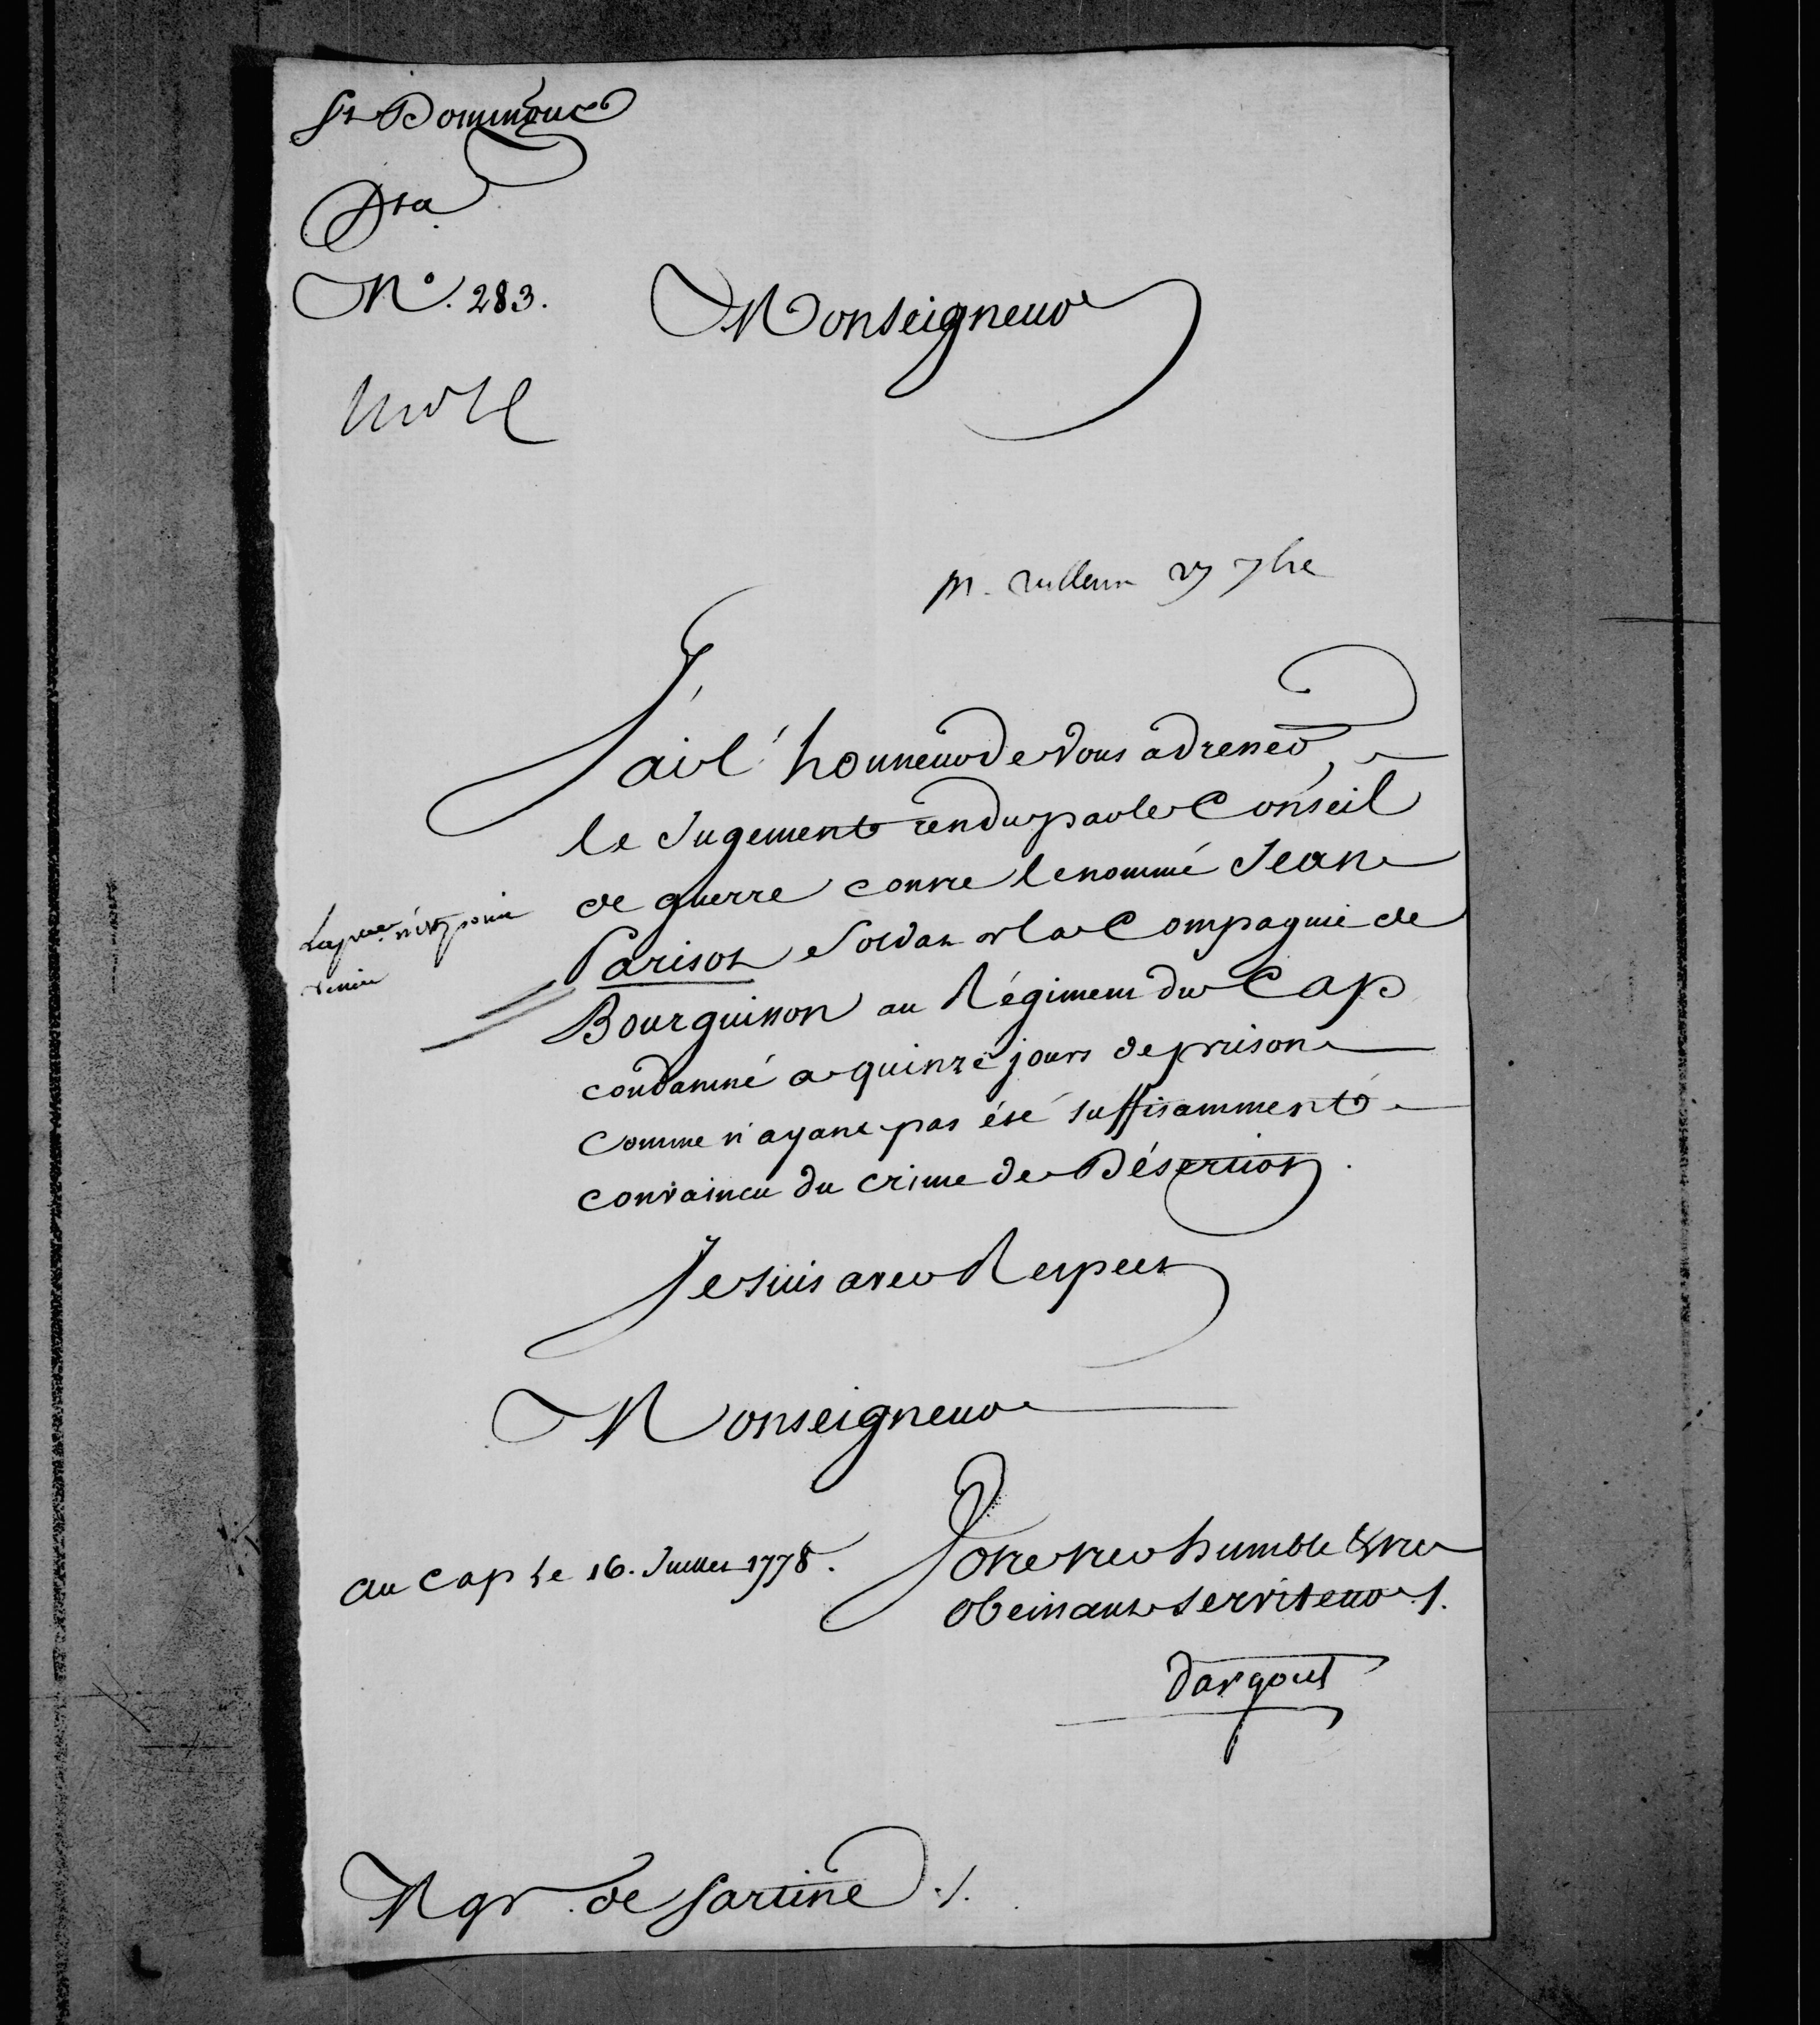
\includegraphics[width=\linewidth,height=6cm,keepaspectratio=false]{images/parisot-lettre-sentence-conseil.jpg}
    \caption{Compte-rendu d'un conseil de guerre, procès de Jean Parisot (ANOM COL E 328bis).}
    \label{fig:parisot-sentence-conseil}
\end{subfigure}
\hfill
\begin{subfigure}{0.32\textwidth}
    \centering
    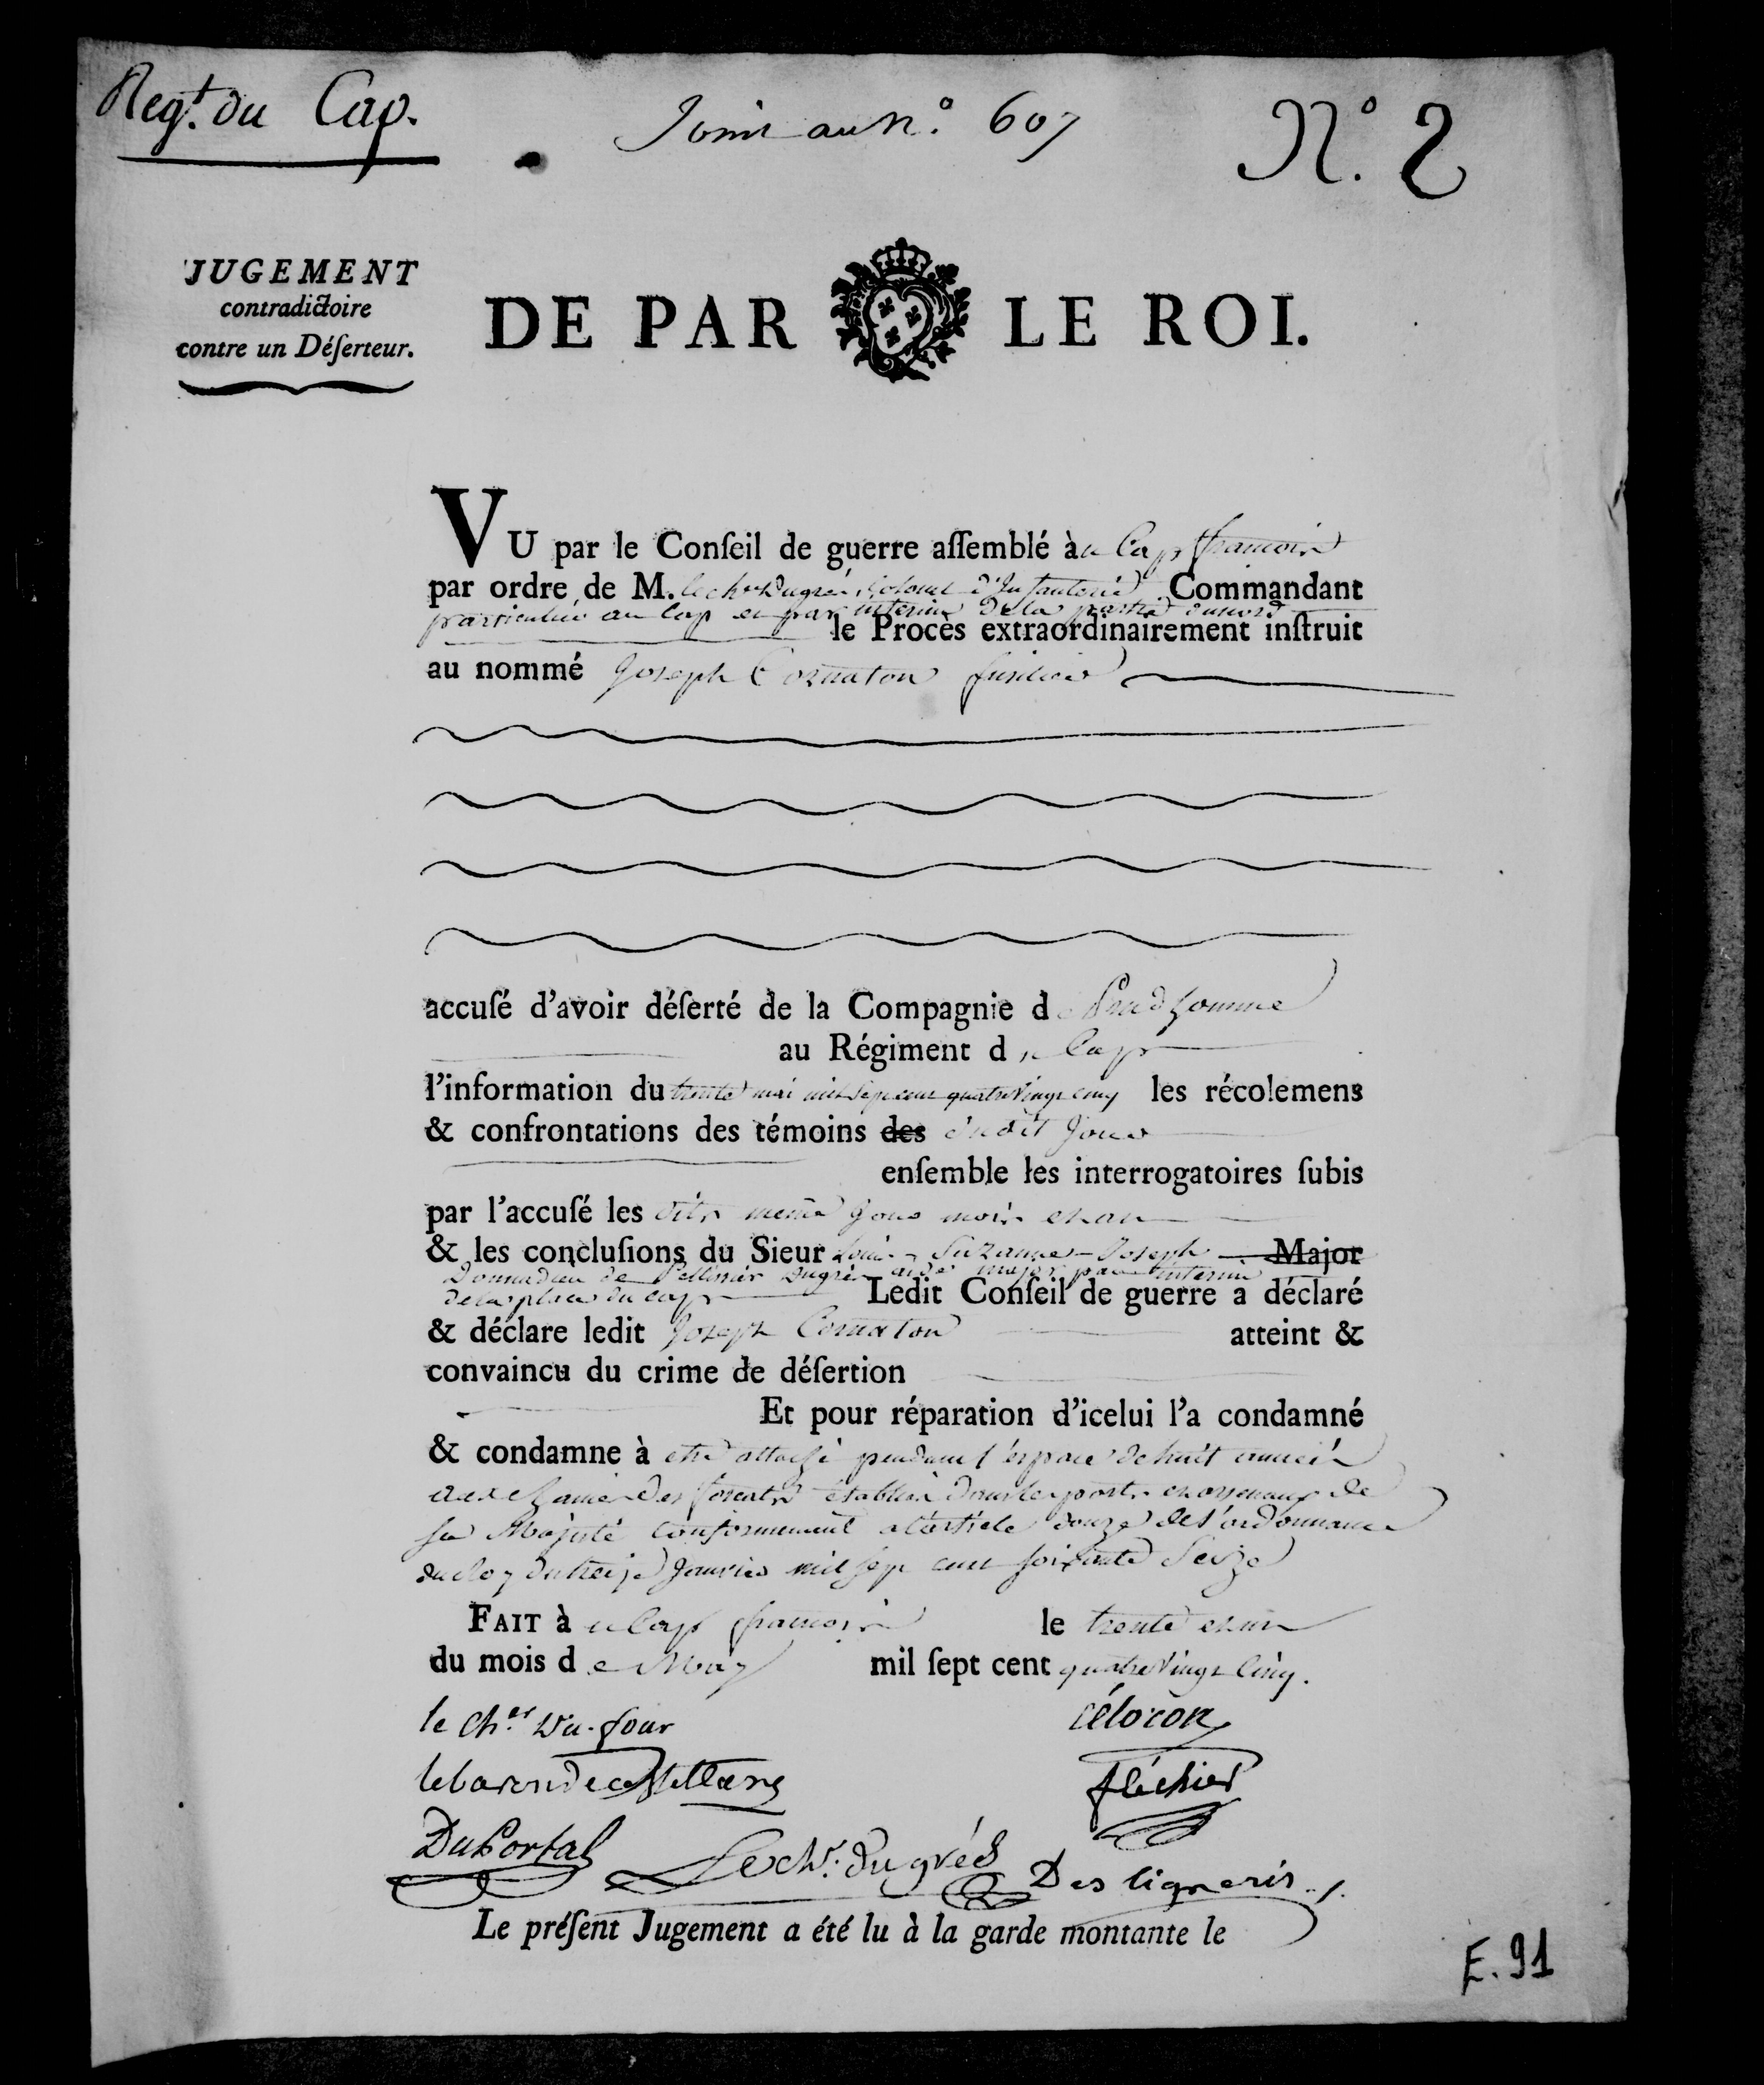
\includegraphics[width=\linewidth,height=6cm,keepaspectratio=false]{images/cornaton-jugement-contradictoire-cole91.jpg}
    \caption{Jugement contradictoire contre un déserteur, procès de Joseph Cornaton (ANOM COL E 91).}
    \label{fig:cornaton-jugmement-contradictoire}
\end{subfigure}
\hfill
\begin{subfigure}{0.32\textwidth}
    \centering
    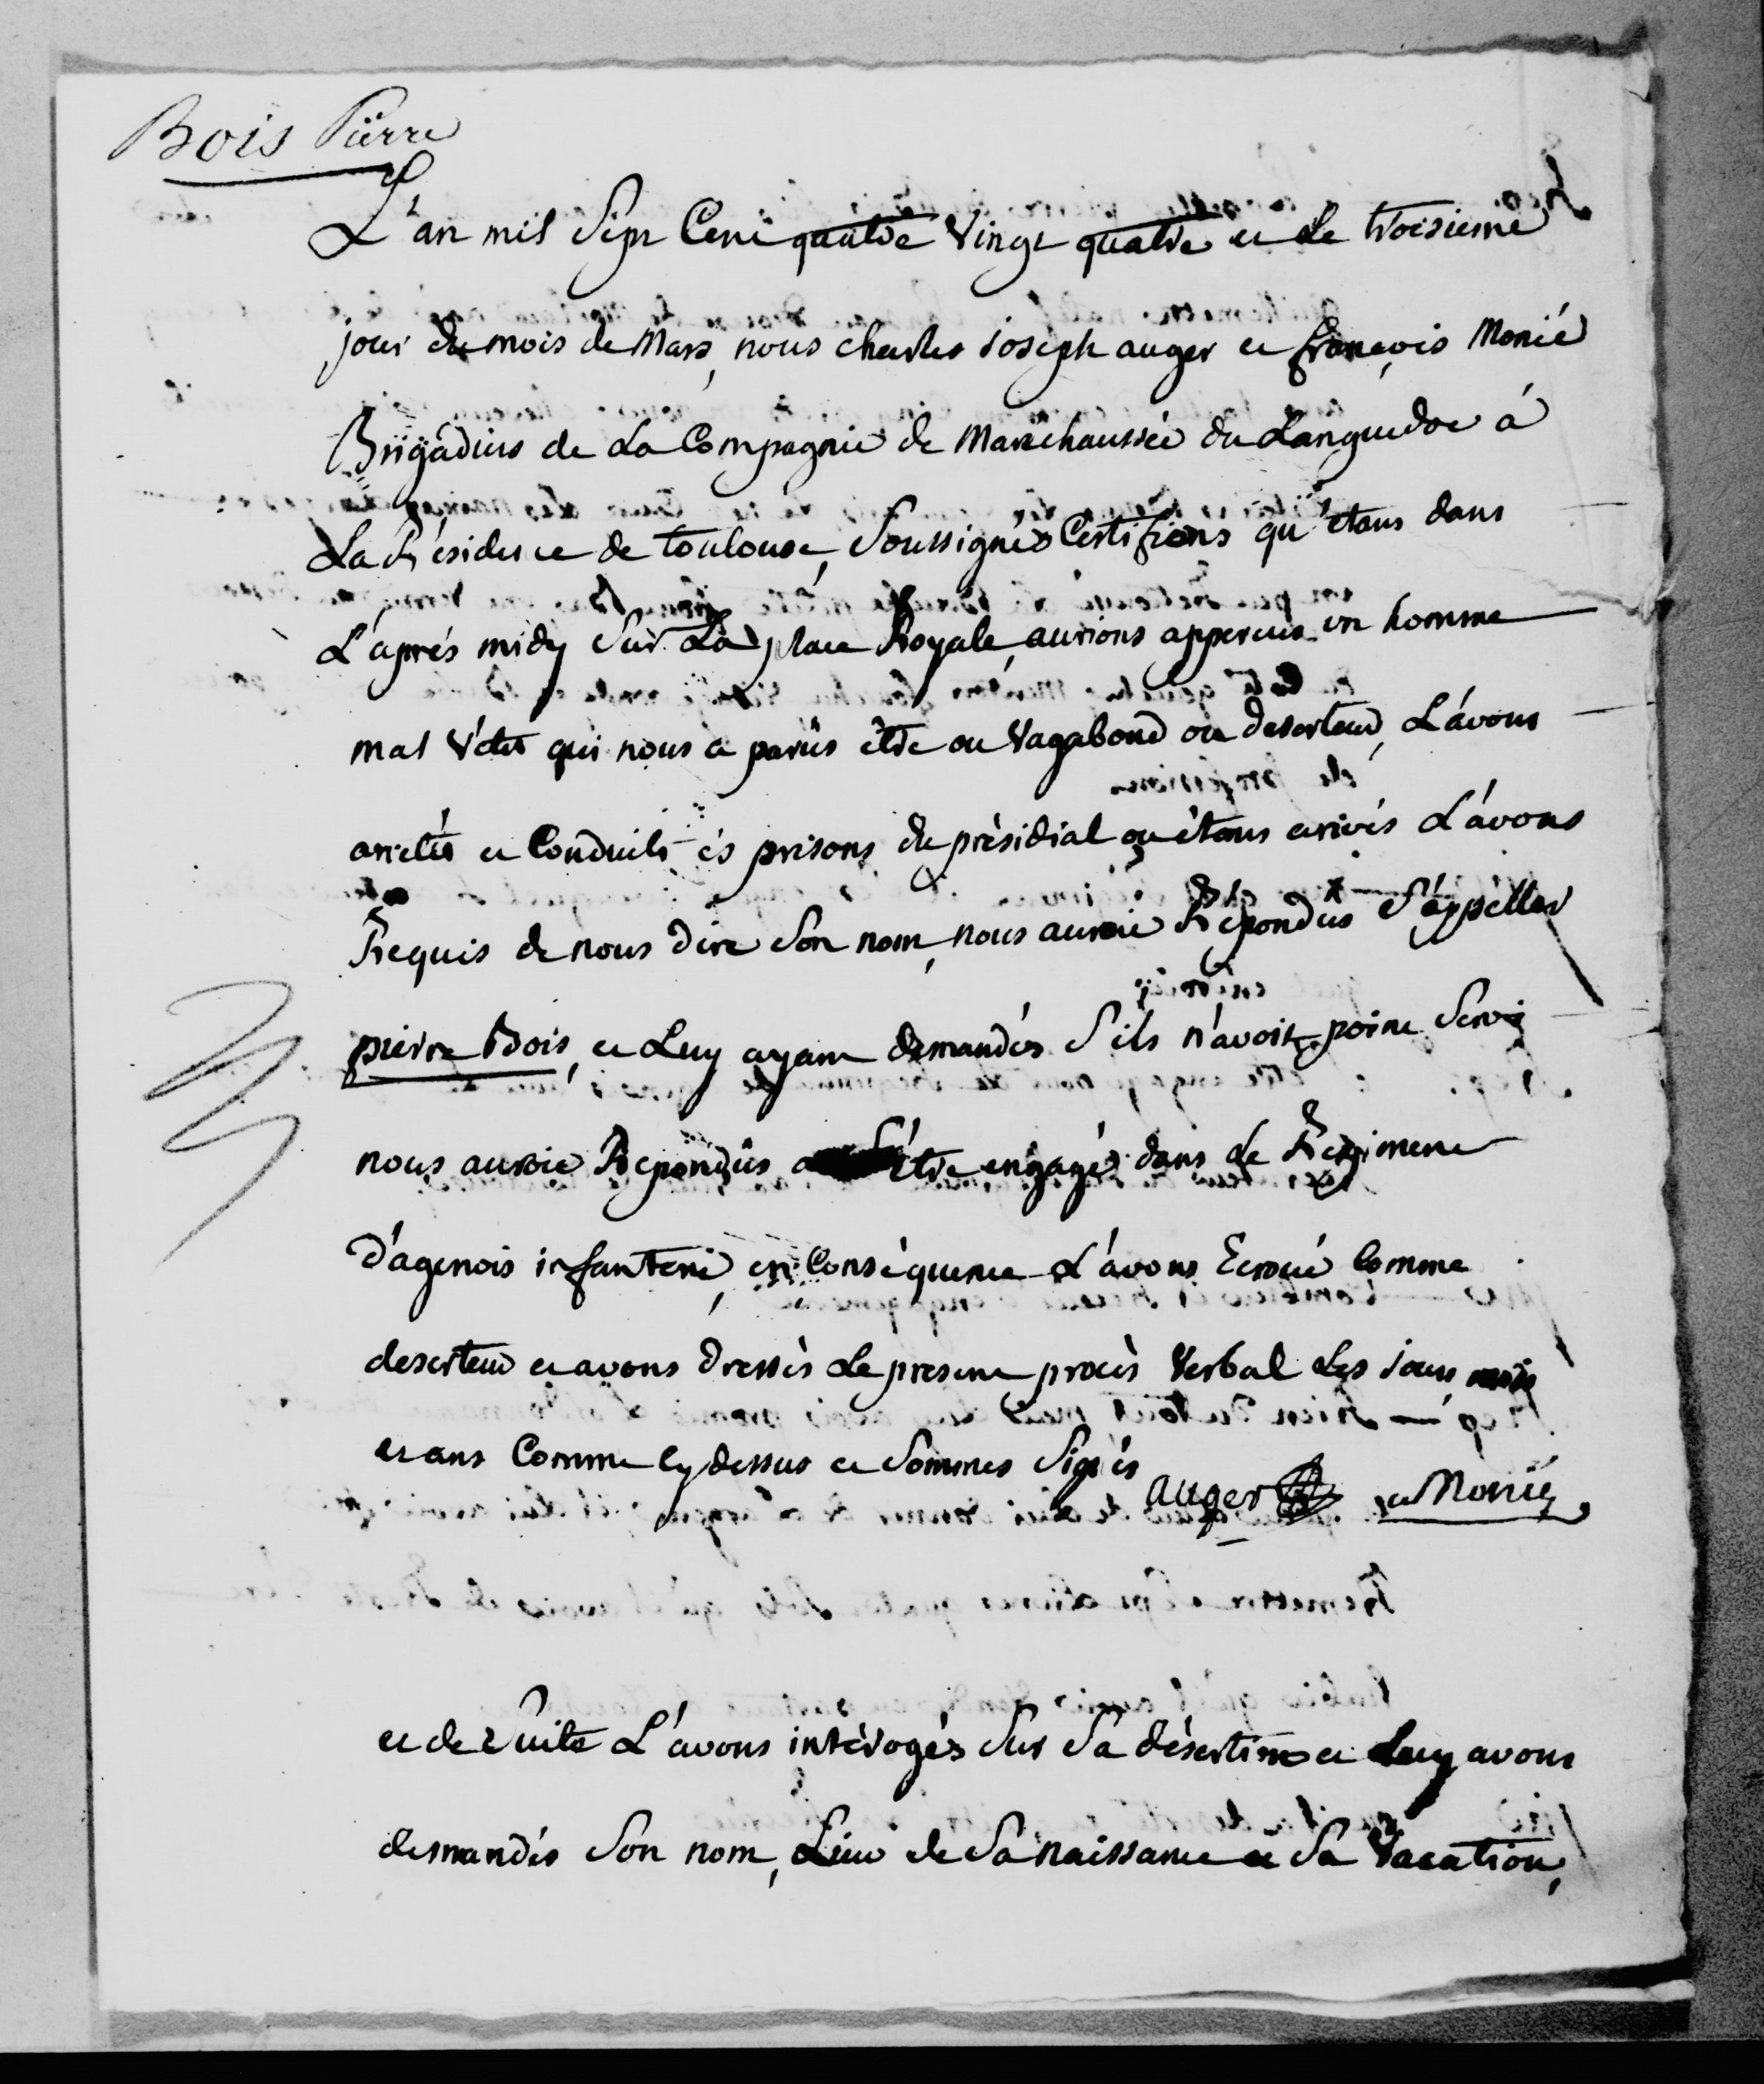
\includegraphics[width=\linewidth,height=6cm,keepaspectratio=false]{images/dubois-pierre-cole140.jpg}
    \caption{Compte-rendu de capture de Pierre Bois, par la maréchaussée (ANOM COL E 140).}
    \label{fig:bois-capture-maréchaussée}
\end{subfigure}

\caption{Exemples de documents contenus dans la COL E des Archives Nationales d'Outre-mer.}
\label{fig:trois_images}
\vspace{.2cm}
\end{figure}

\subsection{Corpus}

Notre volonté de créer un modèle d'ATR dépassant le cadre de ce simple travail, nous avons pris en compte la totalité des dossiers personnels de soldats conservés aux Archives nationales d'Outre-Mer à Aix-en-Provence (ANOM), qui, dans le cadre d'un partenariat de recherche, nous a confié l'intégralité de la série COL E numérisée. Réunie de manière arbitraire par différents archivistes au cours du temps, cette collection contient les dossiers des personnels administratifs, civils et militaires des colonies (comptes, correspondance, mémoires, extraits mortuaires, registres de succession, procès, etc., cf.~fig. ~\ref{fig:trois_images}). Le corpus de travail pour l'ajustement du modèle se compose d'échantillons de trois sous-corpus (Tab.~\ref{tab:corpus}): des extraits de COL E, ainsi que deux corpus de correspondances de planteurs avec leur famille. Les fac-similés retenus pour l'entraînement 
%SG: retenus pour l'entraînement 
ont été choisis de manière à être les plus représentatifs du contenu global des différentes collections.

\begin{table*}[h]
    \centering
    \resizebox{1\linewidth}{!}{
        \begin{tabular}{llcc}
        \hline
        \textbf{Cotes} &\textbf{Type de document} & \textbf{Nombre de vues} & \textbf{Échantillon} \\
        \hline
        ANOM Col E & Dossiers individuels & 351 897 & 449 \\
        AN/T//586 & Correspondance Fougeu-Conflans & 518 & 107 \\
        AN/T//1113 & Correspondance Rochefoucault-Provenchère  & 1181 & 82\\
        \hline
        \end{tabular}
    }
    \caption{\label{tab:corpus}
    Corpus de travail et échantillons retenus pour l'entraînement du modèle d'ATR.
    }
\end{table*}

\subsection{Analyse de mise en page}
À notre connaissance, très peu de projets ont tenté de construire un modèle d'analyse de mise en page pour les documents d'archives de l'époque moderne \cite{koolen_republic_2023,loraine-chappuis-ile-de-france}: nous avons donc tenté de pallier ce problème. La préparation des données pour l'analyse de mise en page a été effectuée grâce à l'application \textit{open source} eScriptorium \cite{escriptorium-an-open-source-platform} dont l'Université de Genève possède une \href{https://www.unige.ch/lettres/humanites-numeriques/recherche/projets/projets-de-la-chaire/fondue}{instance} \cite{fondue-2021}, en suivant les préconisations du projet \href{segmonto.github.io}{SegmOnto} \cite{segmonto-a-controlled-vocsbulary-to-describe-and-process-digital-facsimilies} afin de permettre leur interopérabilité et leur réutilisation \cite{htr-united-a-solution-towards-a-common}. 

\begin{table}[h]
\small
\centering
\begin{threeparttable}
\begin{tabularx}{\textwidth}{
  >{\raggedright\arraybackslash}p{3.5cm}
  >{\centering\arraybackslash}X
  >{\centering\arraybackslash}X
  >{\centering\arraybackslash}X
  >{\centering\arraybackslash}X
  >{\centering\arraybackslash}X
  >{\centering\arraybackslash}X
}
\toprule
\textbf{Zones} &
\textbf{Images} &
\textbf{Nombre d'objets}\tnote{a} &
\textbf{Précision}\tnote{b} &
\textbf{Rappel}\tnote{c} &
\textbf{mAP50}\tnote{d} &
\textbf{mAP50-95}\tnote{e} \\
\midrule
\texttt{all} & 64 & 134 & 62\% & 57.1\% & 52.5\% & 31.6\% \\
\texttt{MainZone} & 64 & 75 & 78.2\% & 88\% & 91.8\% & 65.8\% \\
\texttt{MarginTextZone} & 15 & 22 & 43.6\% & 59.1\% & 41.5\% & 26.8\% \\
\texttt{StampZone} & 20 & 25 & 82.8\% & 92\% & 93.5\% & 54.1\% \\
\texttt{NumberingZone} & 4 & 4 & 73.2\% & 75\% & 68.6\% & 30\% \\
\texttt{DigitizationArtefactZone} & 7 & 7 & 56.1\% & 85.7\% & 67.8\% & 41.8\% \\
DamageZone & 1 & 1 & 0\% & 0\% & 0\% & 0\% \\
\bottomrule
\end{tabularx}

\begin{tablenotes}
\footnotesize
\item[a] Nombre d'objets détectés dans les images.
\item[b] Proportion de détections correctes parmi l’ensemble des détections produites.
\item[c] Proportion d’objets présents qui sont correctement détectés par le modèle.
\item[d] Détection correcte si l’intersection sur union (IoU) entre la prédiction et la vérité terrain est supérieure ou égale à 0,5.
\item[e] Même chose que le précédent, avec des seuils d’IoU allant de 0,50 à 0,95 par pas de 0,05, puis moyennées sur l’ensemble des classes.
\end{tablenotes}
\end{threeparttable}

\caption{Évaluation des performances du modèle \texttt{seg\_megv}.}
\label{tab:description_12}
\end{table}

\begin{wrapfigure}{r}{0.6\textwidth}
    \centering
    \vspace{-.5cm}
    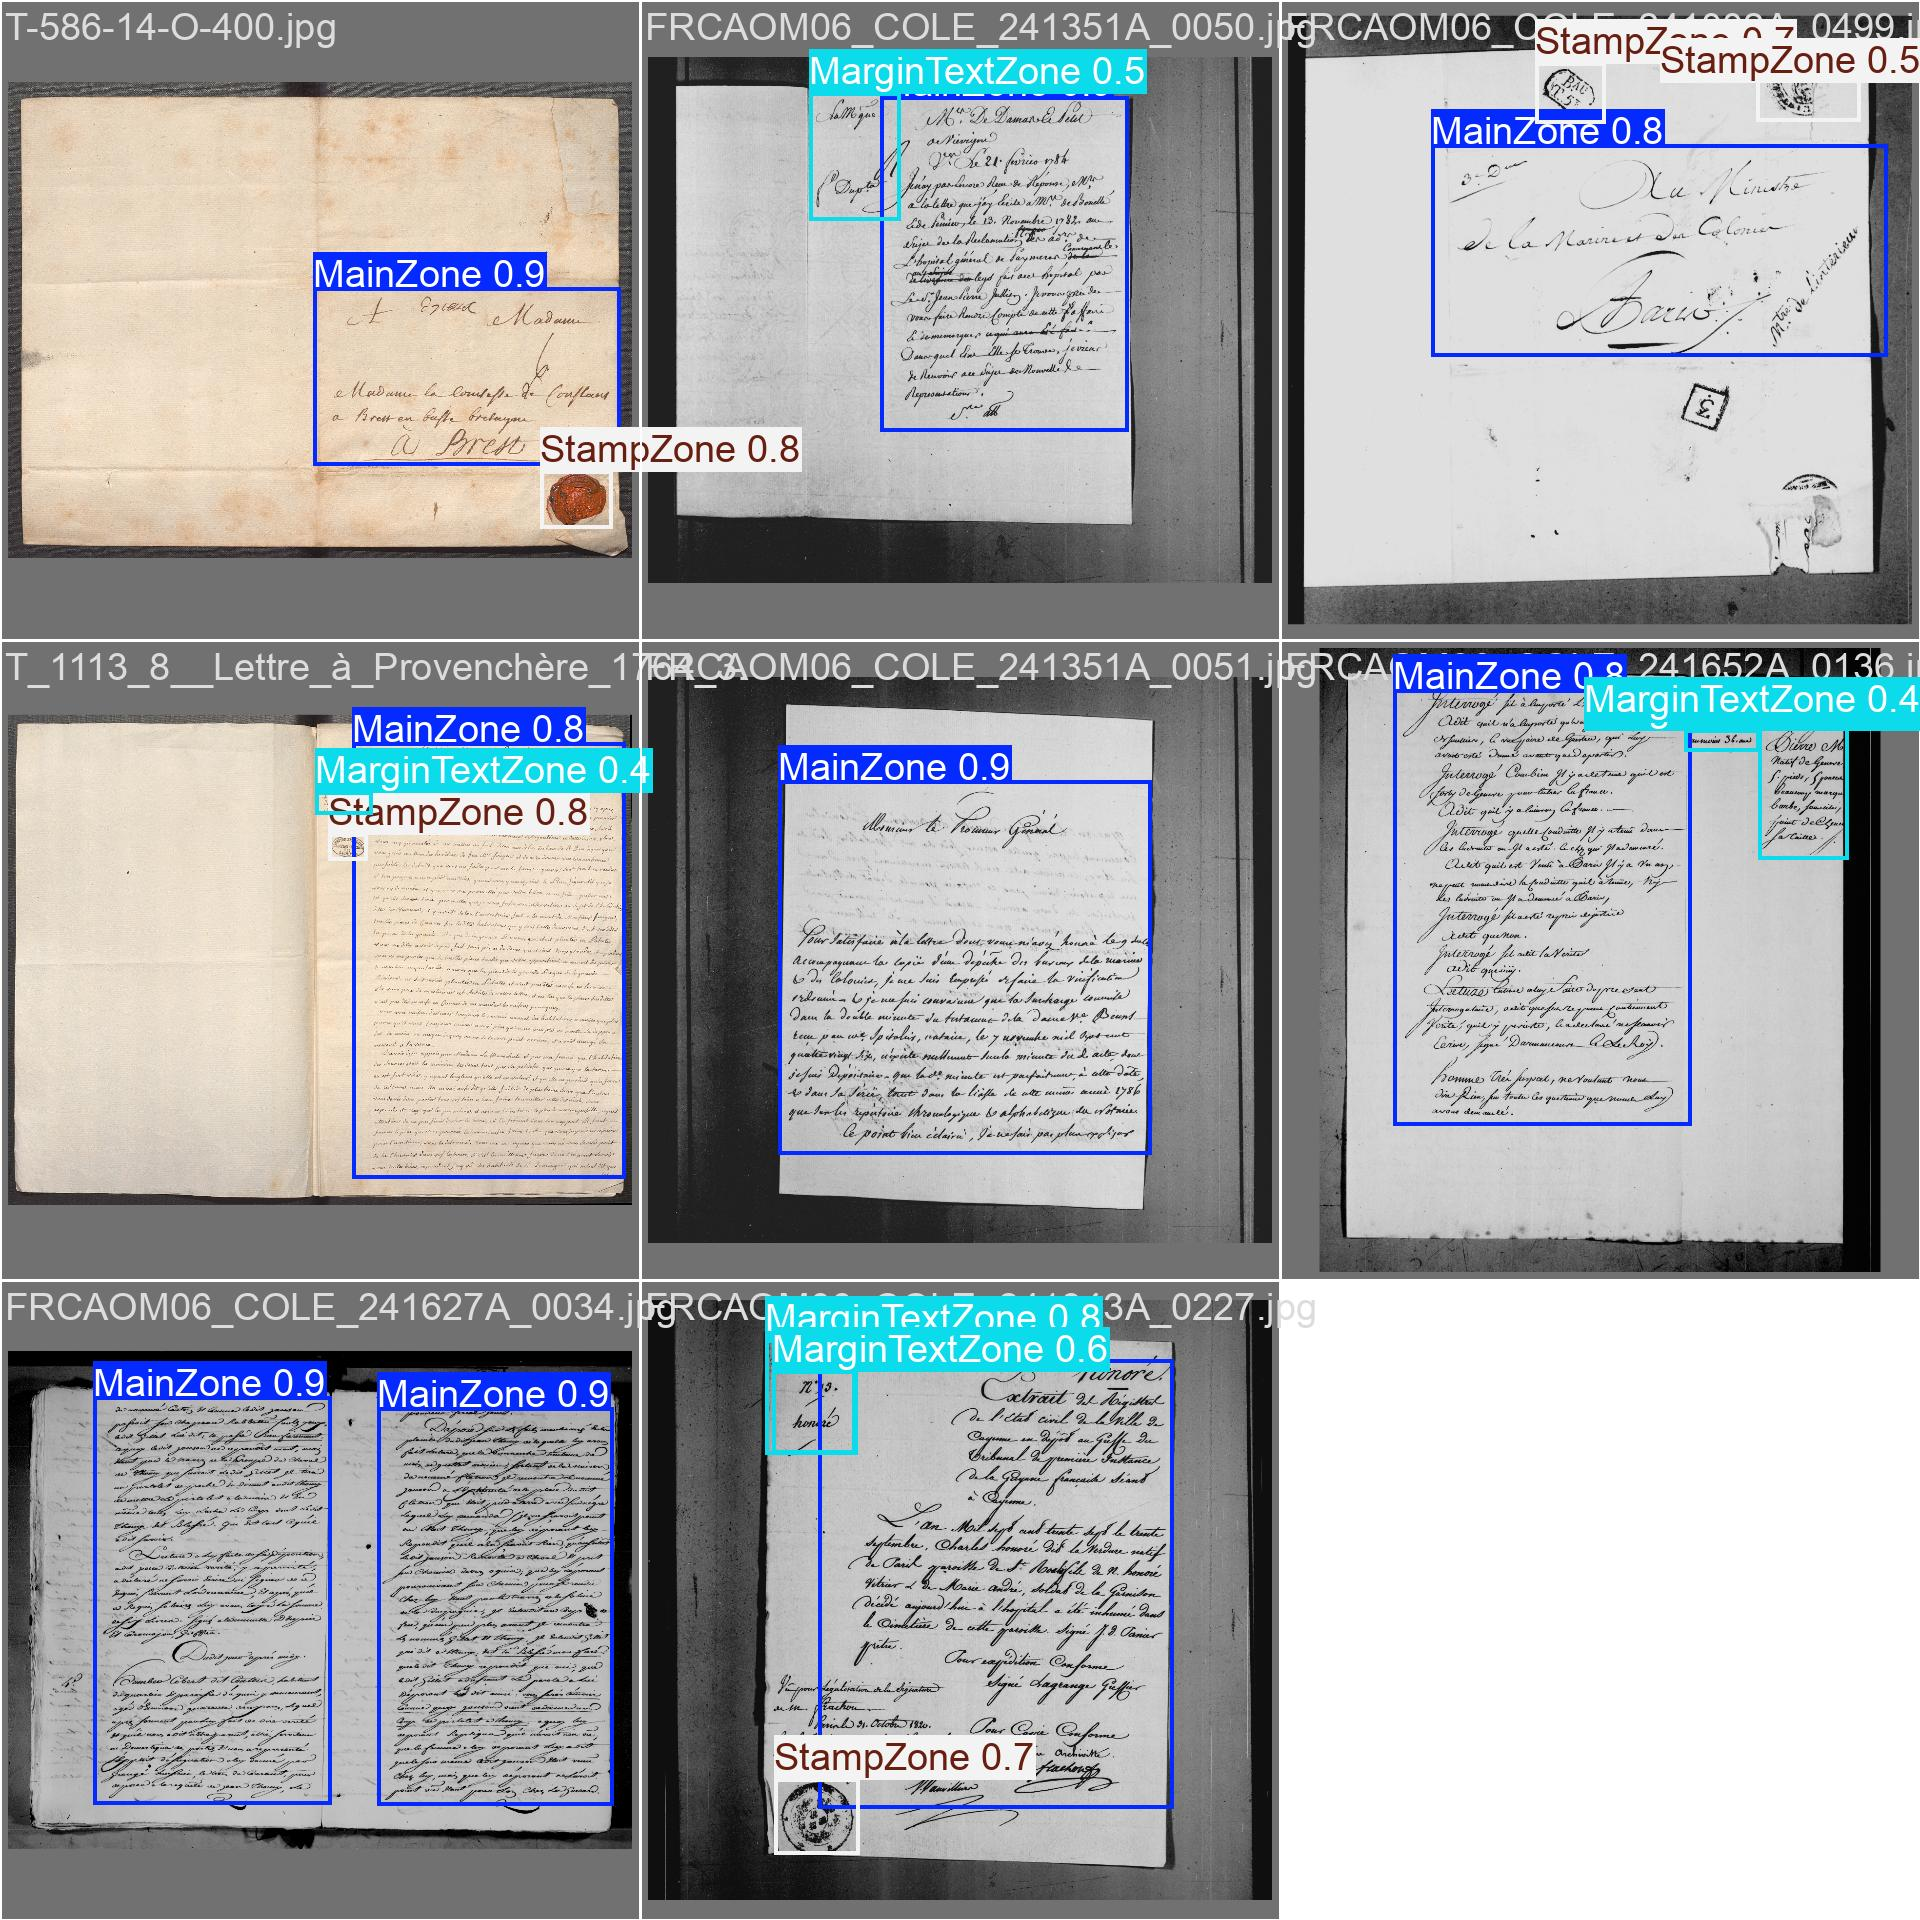
\includegraphics[width=.93\linewidth]{images/val_batch1_pred.jpg}
    \caption{La prédiction faite par le modèle \texttt{seg\_megv}.}
    \label{fig:val_batch1_pred}
    \vspace{-.7cm}
\end{wrapfigure}
Le modèle obtenu, nommé \href{https://github.com/Masculinites-Esclavagistes/MEGV-FR-MSS-18/releases/download/v.2.0.0/seg_megv.pt}{\texttt{seg\_megv}}, 
constitue une première proposition de modèle d'analyse de mise en page pour la pluralité de documents administratifs de l'Empire français à l'époque moderne (Tab.~\ref{tab:description_12}). Pour son entraînement, nous avons identifié six zones (Fig.~\ref{fig:val_batch1_pred}). Le but était qu'elles ne soient pas trop compliquées (afin de distinguer le corps de texte et les marges principalement), mais qu'elles soient aussi communes à tous les types de documents étudiés:
%TC:ignore
\begin{itemize}
    \item \texttt{MainZone}: pour le corps du texte,
    \item \texttt{StampZone}: pour les tampons ou les cachets,
    \item \texttt{NumberingZone}: pour la numérotation des pages, 
\end{itemize}

\begin{itemize}
    \item \texttt{DigitizationArtefactZone}: pour les zones où du texte est récupéré mais ne nous intéresse pas,
    \item \texttt{MarginTextZone}: pour le texte situé en marge du corps du texte,
    \item \texttt{DamageZone}: pour les zones de texte endommagées.
\end{itemize}
%TC:endignore

\subsection{Reconnaissance automatique de texte (ATR)}

Après avoir testé les modèles d'ATR disponibles et en l'absence d'étude sur les mains des administrateurs coloniaux du \textsc{xviii}\textsuperscript{e} siècle, nous avons préparé des données spécifiques pour ajuster (\textit{fine-tune}) le modèle généraliste \texttt{FoNDUE-GD-v3-fr} \cite{transcribing-western-modern-manuscripts}. Concernant le type de transcription des données utilisé pour l'entraînement du modèle ATR, nous avons choisi de suivre les conseils du \textit{Guide pour le traitement numérique des textes en français} \cite{guide-pour-le-traitement-num} afin de permettre l'interopérabilité de ces données, utiles dans l'entraînement des méga modèles \cite{vers-un-modele-diachronique-pour-les-mains-modernes-françaises}. Cette approche a en effet déjà démontré son efficacité dans les travaux de L. Chappuis \cite{loraine-chappuis-ile-de-france} sur les documents conservés aux National Archives of Mauritius, et d'Y. Jauregui \cite{yvan-jauregui-espionner-les-espions} sur les manuscrits de la Bibliothèque de l'Arsenal (tab.~\ref{tab:transcription}).

%TC:ignore
\begin{table*}[htp]
    \centering
    \resizebox{1\linewidth}{!}{
        \begin{tabular}{lllll}
            \toprule
            \textbf{Catégorie} & \textbf{Cas} & \textbf{Traitement} & \textbf{Exemple} & \textbf{Image} \\
            \midrule
            Abréviation & Esperluette (\&) & Conservation & \& & 
\includegraphics[height=1.25em]{images/&.png}\\
            Abréviation & Sommes d'argent & Guillemets droits \texttt{"} (\texttt{U+22}) & 4010\textasciicircum lt {\texttt{"}} {\texttt{"}} & 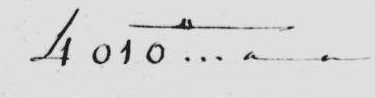
\includegraphics[height=1.25em]{images/4010lt.png}\\
            Abréviation & Suscrites & Précédé de \textasciicircum (\texttt{U+02C6}) & la D\textasciicircum lle & 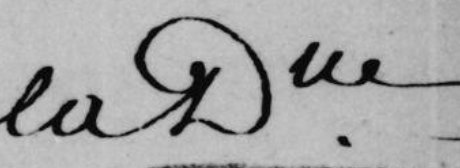
\includegraphics[height=1.25em]{images/Dlle.png} \\
            Agglutination & Pas d'apostrophe & Respect du système & jay lhonneur & 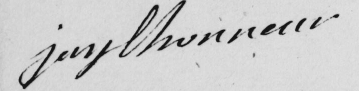
\includegraphics[height=1.25em]{images/jay-lhonneur.PNG}\\
            Signe & Croisettes & Croisettes\ {\fontspec{Noto Serif}※}
※ (\texttt{U+203B}) & intentions\ {\fontspec{Noto Serif} ※} & 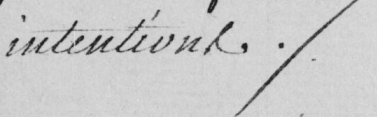
\includegraphics[height=1.25em]{images/intentions.croisette.png} \\
            Correction & Rature lisible & Entre doubles-crochets (\texttt{U+301A} et \texttt{U+301B}) & [[une]] & 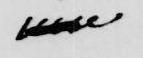
\includegraphics[height=1.25em]{images/une_crochet.lisible_.png}\\
            Correction & Rature lisible & Entre doubles-crochets (\texttt{U+301A} et \texttt{U+301B}) & ses [[...]] & 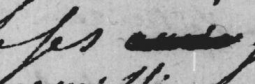
\includegraphics[height=1.25em]{images/ses_crochet.illisible_.png}\\
            \bottomrule
        \end{tabular}
    }
    \caption{\label{tab:transcription}
    Principales règles de transcription.
    }
    \vspace{.2cm}
\end{table*}
%TC:endignore

%Ainsi, 
%SG: les connecteurs en début de paragraphe sont souvent superflus. Allège: retire-le, ça passe tout seul ;-)
Nous avons ajusté le modèle généraliste \texttt{FoNDUE-GDv3-fr} avec nos données, afin de développer un modèle plus adapté aux mains des administrateurs coloniaux du corpus de la COL E, nommé \texttt{FoNDUE-GD-MEGV-v2}. Pour déterminer son efficacité réelle, nous l'avons comparé avec \texttt{FoNDUE-GD-v3-fr}, en les testant tous les deux sur un même jeu de données constitué de 17 folios qui n'ont pas été vus pendant l'entraînement. Le nouveau modèle \href{https://github.com/Masculinites-Esclavagistes/MEGV-FR-MSS-18/releases/download/v.2.0.0/fondue_gd_megv_v2.mlmodel}{\texttt{FoNDUE-GD-MEGV-v2}} 
ajusté spécifiquement pour nos données a permis d'augmenter la performance en exactitude de caractères de 1,48 pt de \% et d'augmenter de 4,92 pt de \% la performance en exactitude mot à mot \cite{rapport-d-etape-megv}
(Tab.~\ref{tab:description_modèles_efficacité}). Il constitue à ce jour le premier modèle d'envergure ciblé sur un corpus de documents privés et administratifs de l'Empire français.

\begin{table}[h]
\centering\small
\begin{tabular}{p{4cm}p{3.1cm}p{3.1cm}p{3.1cm}} % p{} pour permettre les retours à la ligne
\toprule
\textbf{Modèle testé} & \textbf{Nombre d'erreurs} & \textbf{Exactitude de caractères} & \textbf{Exactitude mot à mot}\\
\midrule
\href{FoNDUE-GD-v3-fr}{FoNDUE-GD-v3-fr}& 4422 & 81,81\% & 46,65\% \\ \midrule
\href{https://github.com/Masculinites-Esclavagistes/MEGV-FR-MSS-18/releases/tag/v.2.0.0}{FoNDUE-GD-MEGV-v2} & 4062 & 83,29\% & 51,57\% \\ \bottomrule
%FoNDUE-GD-MEGV-v2 & 4062 & 83,29\% & 51,57\% \\ \bottomrule
\end{tabular}
\caption{Évaluation des différents modèles sur un lot de 17 fac-similés numériques.}
\label{tab:description_modèles_efficacité}
\end{table}


\section{Méthode}

Pour notre corpus de travail, nous avons sélectionné 185 dossiers de soldats via une recherche par mots-clés dans leur titre dans l'inventaire de la série COL E. 
%Nous avons appliqué les modèles d'ATR et de segmentation obtenus sur ces 185 dossiers de déserteurs, et nous avons généré des fichiers .xml et .tei, transformés via un script xslt afin de produire une page html 
%SG: 
Nous avons appliqué les modèles d'ATR et de segmentation obtenus sur ces 185 dossiers de déserteurs: les fichiers ALTO ont été successivement transformés en TEI et en HTML grâce à des feuilles de style XSLT, permettant l'affichage simultané des sources et de leur transcription
\footnote{Nous remercions Fl. Goy et M. Philip 
pour leur aide dans la création du script xslt.} (fig.~\ref{fig:html-cornaton}).
Grâce à une recherche par mots-clés effectuée dans cette page html, puis complétée par une recherche manuelle lorsque cela a été nécessaire en raison du manque de précision de l'ATR, les dates de désertion présentes dans 127 dossiers ont été retenues.
%afin d'étudier la répartition chronologique de la désertion dans les colonies françaises de la Caraïbe au cours du \textsc{xviii}\textsuperscript{e} siècle.

\begin{figure}[h]
    \centering
    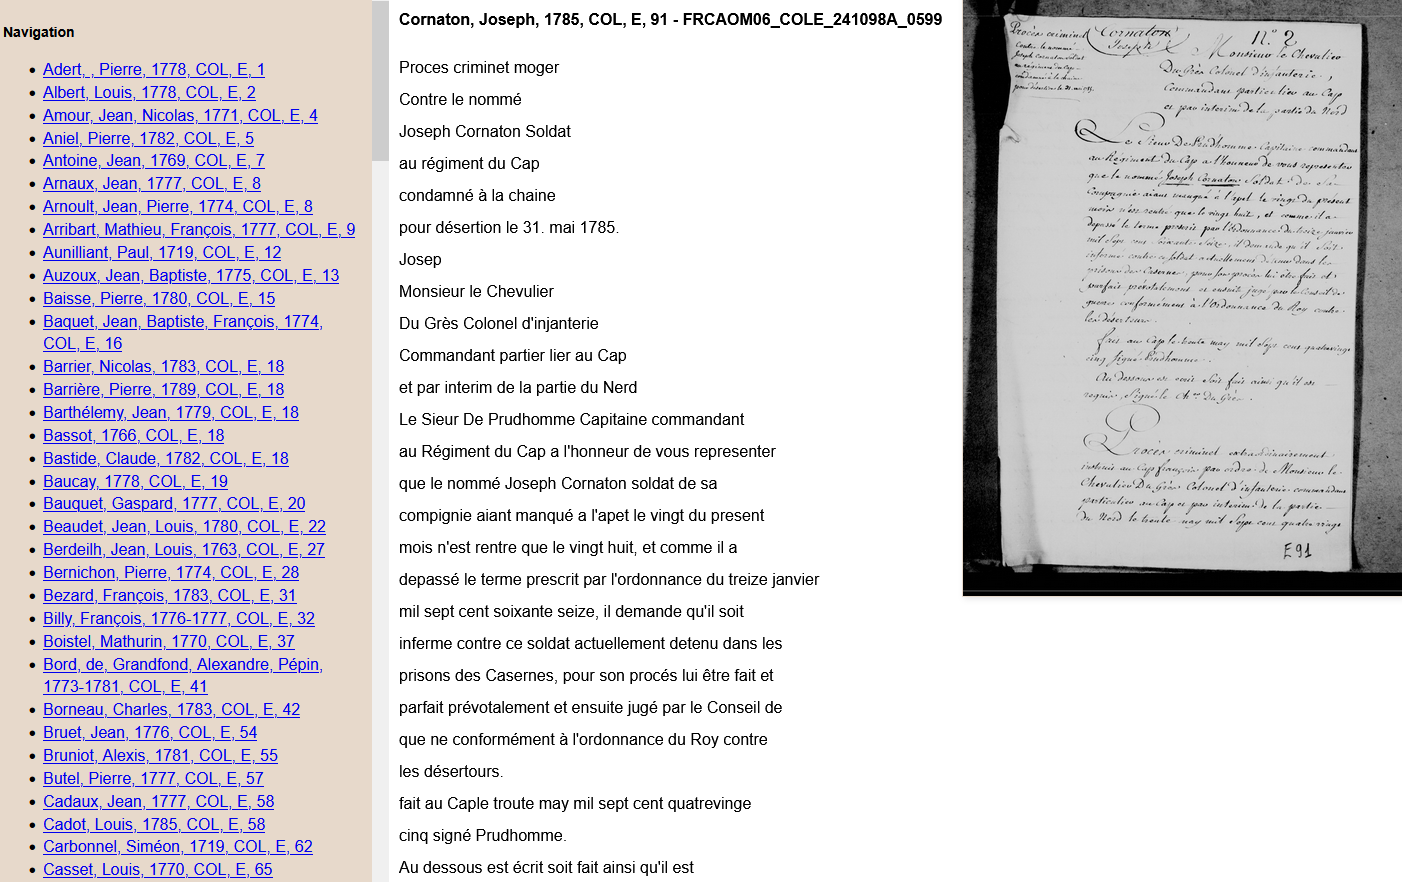
\includegraphics[width=1\linewidth]{images/html-cornaton.PNG}
    \caption{Capture d'écran de la page html produite.}
    \label{fig:html-cornaton}
    \vspace{.5cm}
\end{figure}

Cet écart entre les 185 dossiers initiaux et les 127 conservés est expliqué par les cas non-retenus de soldats déserteurs en métropole, rattrapés et envoyés servir pour une certaine durée dans les troupes coloniales, en échange de la commutation de leur peine. Dans la mesure où la désertion ayant eu lieu en métropole est bien connue à l'époque moderne \cite{corvisier_armee_1964,seriu2005}, ces 58 cas ont été volontairement écartés pour nous concentrer sur ceux arrivés sur le terrain colonial, en raison de ses particularités géographiques (insularité) et techniques (éloignement de la métropole de plusieurs mois de navigation, dynamiques sociales en société esclavagiste). 

\section{Résultats}

Le résultat obtenu est un graphique montrant le nombre de désertions par année (1696-1790), en fonction des colonies, prenant en compte au total les 127 cas pertinents contenant au moins une année de désertion déclarée (Fig.~\ref{fig:desertions-annee}). 

\begin{figure}[ht]    
        \centering
        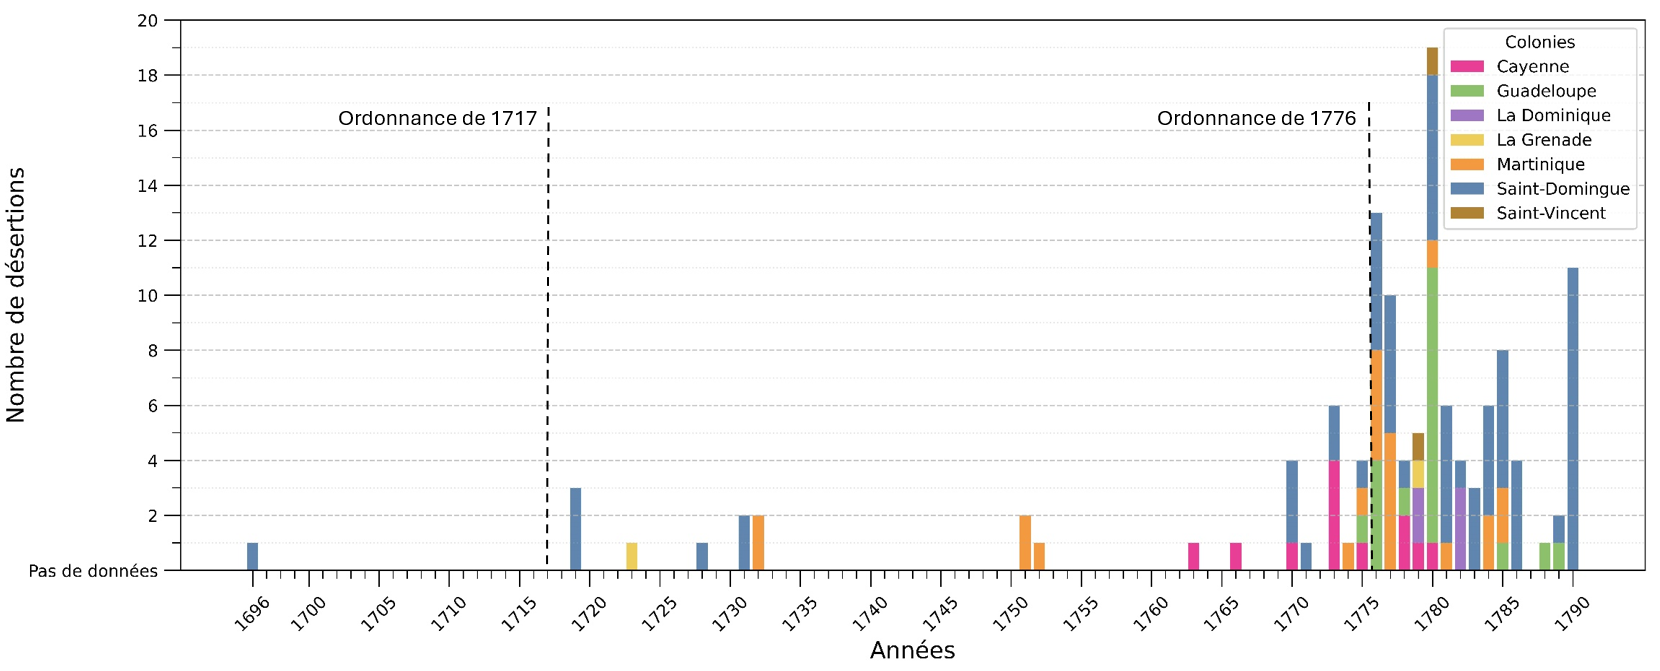
\includegraphics[width=1\textwidth]{images/Nombre de désertions par an par colonie_ordonnances.jpg}
        \caption{Nombre de désertions par an (1696-1790) en fonction des colonies.}
        \label{fig:desertions-annee}
    \vspace{.2cm}
\end{figure}

Le siècle est marqué par deux ordonnances majeures contre la désertion: celle de 1717 transforme la peine des galères initialement prévue en peine de mort, tandis que celle de 1776 transforme la condamnation à mort en travaux forcés, selon les circonstances et le moment de la désertion, et émet par la même occasion une amnistie pardonnant les déserteurs partis avant le 1er janvier 1776 qui se présenteront \footnote{\textit{Ordonnance du Roy, portant amnistie générale […] 1716, op. cit.}; et \textit{Ordonnance du Roi, qui accorde amnistie aux déserteurs de la Marine et des Colonies, du 13 janvier 1776}, in Moreau de Saint-Méry, Lois et constitutions des colonies françoises de l'Amérique sous le Vent, Paris, Moutard imprimeur, 1784-1790, t.~5, p.~658.}. D'emblée, nous pouvons constater dans l'ensemble une corrélation entre le changement juridique apporté par l'ordonnance de 1776 et le changement dans la pratique de désertion. Il est malheureusement difficile de se prononcer sur un potentiel effet de l'ordonnance de 1717 sur le comportement des hommes. Le peu de cas de la première moitié du \textsc{xviii}\textsuperscript{e} siècle et leur grand nombre pour la fin du siècle peuvent être expliqués par des dynamiques matérielles de conservation des documents, en élaboration tout au long du siècle \cite{Houllemare-archives-imperiales}. En revanche, le pic des désertions de la fin du siècle coïncide avec l'ordonnance de 1776 qui supprime la peine de mort au profit des travaux forcés. Ainsi, la superposition de ces deux phénomènes pour la fin du siècle semble montrer que la loi est connue des hommes, qui profiteraient de son relâchement pour partir: elle a un effet direct sur les pratiques de désertion.
%SG: là faut faire gaffe. Ce que montre le graphique n'est pas l'effet de l'un sur l'autre, mais une superposition des deux phénomènes. L'effet tu le déduis, et donc tu le prouves.


À l'échelle des colonies, il est frappant de constater que la moitié des cas de désertion ont lieu à Saint-Domingue. Cette particularité peut être due à plusieurs facteurs. Beaucoup plus grande que les autres, Saint-Domingue accueille davantage de soldats en garnison, ce qui peut expliquer qu'il y ait proportionnellement plus de cas. Ensuite, les intérêts économiques de la France dans cette colonie sont très forts. Première productrice de sucre, elle importe énormément d'esclaves, et ses dynamiques sociales sont marquées par un climat de violence général beaucoup plus fort que dans les autres colonies esclavagistes des petites Antilles \cite{Rogers_raciser_la_société,butel-histoire-des-antilles}. D'ailleurs, dès la fin des années 1770, elle devient une place centrale pour l'accueil des détachements et des escadres français envoyés pour combattre lors de la Guerre d'Indépendance américaine \cite{lesueur_troupes_2009}. S'il est impossible de relever les tendances de désertion dans la Caraïbe lors de la Guerre de Sept Ans (1756-1762), l'arrivée de la guerre semble pourtant constituer un facteur externe et interne fort: l'optique de se battre réellement et de risquer sa vie autrement que dans les garnisons et les travaux pour son compte ou celui du Roi amène aussi les hommes à fuir. Ainsi, la prépondérance de la colonie de Saint-Domingue dans les cas de désertion peut s'expliquer tant par des facteurs structurels des sociétés esclavagistes, que des facteurs internes propres aux dynamiques sociales de Saint-Domingue et des facteurs externes, tels que la réalité de la guerre.
%SG: attention à la phrase à tiroirs multiples


\section{Discussion}

%Selon les 
%SG: sur la base des
Sur la base des résultats observés, il est possible d'affirmer que les soldats ont une bonne connaissance des réformes législatives qui les concernent. Cependant, il faut être attentif au fait que cette lecture distanciée de sources judiciaires reflète une pluralité de cas individuels
%, 
%SG: si les deux éléments coordonnés ont le même sujet on ne met pas de virgule. Il me semble avoir vu le cas ailleurs.
et appelle une lecture serrée qui permet de mieux comprendre le problème posé par la norme et son appropriation par les subalternes. 

À Saint-Domingue, Gilbert Pépin et Joseph Cornaton, deux soldats de seize ans de la garnison du Cap, partent en 1785 laver leur linge dans la colline voisine. Alors qu'ils boivent ensemble une bouteille d'alcool, ils s'endorment et manquent l'appel du soir à la garnison, ce qui provoque la plainte du capitaine et initie la procédure du jugement pour désertion contre eux. Interrogé \og s'il n'est pas informé de la rigueur des ordonnances du Roy contre les déserteurs \fg{}, Cornaton conteste l'accusation de désertion et répond \og que le jour où elles ont été lues aux casernes il était de garde au fort Picolet, et qu'il croyait seulement qu'il suffisait de ne point passer les limites pour ne pas être réputé déserteur \fg{}\footnote{ANOM COL E 91 et 333.}. 

%Quelques années plus tard, au même endroit, Jean Parisot, natif de Franche-Comté, est quant à lui appréhendé alors qu'il usait d'un droit de promenade qu'il pensait acquis: \og Il fit la rencontre d'un caporal de deux fusiliers qui s'avancèrent vers lui en lui demandant qui il était et où il allait, à quoi il répondit qu'il était soldat au régiment du Cap et qu'il ignorait le lieu ou il allait [...]~; surquoi ils l’arrêtèrent et le conduisirent en prison, ce qui l'a fort étonné n'ayant aucune intention de déserter [...] et que d'ailleurs, il ne croyait pas avoir besoin de permission pour aller se promener \fg{}\footnote{ANOM COL E 328bis.}.
%SG: si tu dois gagner des mots, retire ce second cas, qui fait un peu doublon avec le précédent. Tu le remettrais pour une version longue si tu décides de te lancer!

Cependant, ces cas sont placés dans le graphique sur le même plan que des désertions motivées et parfois avouées, telle la désertion de Jean Diavet, 26 ans, qui s'enfuit en 1776 après 15 mois de service au Cap, affirmant \og n'avoir rien fait que de courir les grands chemins pour arriver le plus tôt possible sur le territoire espagnol \fg{}, afin de se soustraire de l'autorité impériale française\footnote{ANOM COL E 134.}.

Ainsi, si la corrélation entre l'évolution de la loi et l'augmentation de la désertion visible sur le graphique nous permet de penser que les hommes connaissent le cadre juridique qui les concerne et qu'il a une influence sur le choix de la fuite, l'analyse multiscalaire nuance cette hypothèse. Sans remettre en question la tendance globale, l'étude des cas individuels amène à questionner la définition de la désertion, entre définition juridique fixe, compréhension par les soldats et qualification des cas par les autorités \cite{bascoul-colloque-angers}. Sont considérés comme déserteurs devant la justice ceux qui entreprennent réellement de prendre la fuite, tout comme ceux dont le comportement inadapté n'entre pas en adéquation avec la norme.

%Graphique qui montre corrélation entre loi et augmentation de la désertion. Hypothèse des hommes qui connaissent la loi qui les concerne, analyse multiscalaire qui nuance cette affirmation, car necessité de se rapprocher de l'échelle ind pour observer une réelle connaissance ou pas. Et désertion a des contours flous, entre définition juridique fixe, compréhension de cette définition par les soldats et qualification des cas par les autorités : sont considérés comme déserteurs devant la justice ceux qui entreprennent réellement de prendre la fuite, tout comme ceux dont le comportement inadapté n'entre pas en adéquation avec la norme. %\cite{bascoul-colloque-angers}.

%L'analyse multiscalaire permet de constater que les soldats connaissent la loi: ils jugent du moment le plus opportun pour leur départ en fonction des risques encourus, mais aussi en fonction de facteurs internes, propres à la colonie ou externes, tel que l'approche du conflit militaire. Ce constat est cependant à nuancer lorsque l'on se rapproche de l'échelle individuelle, car la désertion est un crime qui dans la pratique dispose de contours flous: sont considérés comme déserteurs devant la justice ceux qui entreprennent réellement de prendre la fuite, tout comme ceux dont le comportement inadapté n'entre pas en adéquation avec la norme. %\cite{bascoul-colloque-angers}.

%SG: c'est pas l'analyse multiscalaire. L'analyse multiscalaire ne permet pas d'affirmer, mais de nuancer une premipre affirmation
%SG: la compréhension est chaotique. Tu dois clarifier. Si je comprends bien, tu repars dans ce paragraphe de la visualisation (et tu répètes donc une affirmation faite dans la partie précédente, ce qui n'est pas forcément utile: je retirerais). Ensuite tu expliques que le changement d'échelle, en passage d'un niveau global à un niveau personnel, permet de nuancer le propos. Cette nuance permet, sans remettre en question une tendance globale, de questionner la définition de la catégorie de désertion, et d'observer un hiatus entre une définition juridique (celle de l'analyse distante) et sa compréhension (celle des études de cas) qui permet de mettre en valeur la diversité des cas. Attention: si tu vas au tribunal (j'ai deux frères avocats), les types ont toujours des explications à ce qu'ils font. Est-ce que la désertion à des contours flous, ou est-ce que les types ont tout intérêt à "flouter" les contours pour expliquer que c'est pas leur faute quand ils se font attraper?

\section{Pistes}
Ce travail permet ainsi de contribuer à l'étude des réactions individuelles face aux changements dans le droit. L'approche distante permet de postuler une corrélation entre changement de la loi en 1776 et modification des comportements, les études de cas permettant d'améliorer la compréhension de ces derniers. La collecte des données a fait émerger des tendances de désertion qui restent à exploiter, telle que le choix de la journée comme moment privilégié de la fuite, ou la répartition annuelle des cas de désertion.
%Si notre graphique représente la désertion dans un sens large, sa réalisation a permis de constater au plus près des sources des tendances insoupçonnées et surprenantes.
%SG: là c'est trop flou et un peu trop "effet wow". Reprenons ma proposition du début, à savoir de développer l'apport méthodologique – l'apport historique étant selon moi clair avec la partie précédente: "Ce travail permet ainsi de contribuer à l'étude des réactions individuelles face aux changements dans le droit. L'approche distante permet de postuler une corrélation entre changement de la loi en 1776 et modification des comportements, les études de cas permettant d'améliorer la compréhension de ces derniers. Le mouvement de redescente est donc fondamental
%Il révèle que sur les quatorze cas mentionnant un moment de la journée pour la fuite, huit ont lieu en plein jour, et non pas au couvert de la nuit pour masquer la fuite, ou encore que la répartition temporelle des désertions au sein de l'année est très large, les déserteurs ne fuyant pas toujours durant la bonne saison. 
%SG: tu devrais thématiser qu'il s'agit d'une première exploration mais que des données restent à exploiter.
Finalement, cette analyse temporelle nous a permis d'identifier des groupes de désertions différents, révélant que certains hommes ont choisi la fuite en groupe plutôt que la fuite individuelle. 

De tels résultats encourageants et permis par la lecture distante incitent à approfondir notre analyse des dynamiques globales du moment de la désertion, en se concentrant sur des analyses micro-historiques, afin de questionner les dynamiques sociales, les stratégies et les relais de la fuite.  %Dans cette optique, le modèle ATR utilisé nécessite d'être amélioré afin de l'appliquer sur un plus grand nombre de dossiers et y découvrir ceux qui ont mal été classés et qui concernent pourtant d'autres soldats déserteurs invisibles jusqu'à maintenant dans le corpus. 

%\section*{Remerciements}

%Merci à Simon Gabay, Marion Philip, Méloé Maillard et Marie Houllemare pour leur relectures et conseils. 


\section*{Financement}

Les recherches ont été menées dans le cadre du projet \textit{Masculinités esclavagistes} (FNS \href{https://data.snf.ch/grants/grant/219753}{\underline{n° 219753}}).

% Imprime la bibliographie à la fin. Gardez cette ligne après le texte
% principal de votre article et avant une annexe.
\printbibliography
% Vous pouvez inclure une annexe en utilisant la commande suivante
%\appendix
%\section{Première section de l'annexe} \label{appdx:first}
%Des annexes facultatives peuvent être ajoutées après la section des références. 
\end{document}